\documentclass[sigconf, nonacm]{acmart}

\settopmatter{printacmref=false}
\setcopyright{none}
\renewcommand\footnotetextcopyrightpermission[1]{}
\pagestyle{plain}

\usepackage{booktabs}
\usepackage{graphicx}
\usepackage{subcaption}
\usepackage{enumitem}

\begin{document}

\title{Predicting UAV Flight Path Deviation from Onboard Telemetry and Wind
Conditions Using Interpretable Machine Learning}

\author{Abdulaziz Al-Haidary}
\email{alhaidaryaa@g.cofc.edu}
\affiliation{%
  \institution{College of Charleston}
  \city{Charleston}\state{SC}\country{USA}}

\author{Azizbek Nurmatov}
\email{nurmatova@g.cofc.edu}
\affiliation{%
  \institution{College of Charleston}
  \city{Charleston}\state{SC}\country{USA}}

\begin{abstract}
Unmanned aerial vehicles flying pre-planned survey patterns drift off
their intended track whenever wind overpowers the autopilot's ability to
compensate, degrading the quality of downstream products such as
orthomosaics and soil-moisture maps.  We study cross-track deviation on
15 real outdoor flights of a multi-rotor UAV flown by Dr.\ Hemanth
Dakshinamurthy's group at SC~State University, framed as both
instantaneous regression (deviation in metres) and high-deviation
classification (75th-percentile threshold).  We compare three
interpretable course-covered models (decision tree, $k$-nearest
neighbors, random forest) across \emph{three} families of features:
hourly public weather (Open-Meteo reanalysis), onboard ArduPilot
telemetry (attitude, motor output, rates, vibration, EKF innovations),
and the union of the two.  Evaluated under 5-fold GroupKFold
cross-validation that holds out entire flights, onboard telemetry yields
the best regression ($R^2=0.52$) and the best classification ($F_1=0.89$)
whereas hourly public weather alone gives $R^2<0$ --- actively worse than
a mean predictor.  Feature-importance analysis identifies altitude, EKF
horizontal innovation, and ground speed as the dominant onboard
predictors, consistent with the view that a multi-rotor's own flight-state
telemetry is a better high-frequency wind-response sensor than any
off-board anemometer we could realistically access.  We release the
pipeline at \url{https://github.com/iihakk/-uav-flight-path-deviation-ml}.
\end{abstract}

\keywords{unmanned aerial vehicles, flight path deviation, ArduPilot
telemetry, decision trees, random forest, feature engineering, GroupKFold}

\maketitle

\section{Introduction and Background}

\subsection{Problem}
Unmanned aerial vehicles (UAVs) are now routinely used for precision
agriculture, disaster surveying, and hyperspectral remote sensing, where
strict adherence to a planned flight path is critical to the quality of
downstream products such as orthomosaics, soil-moisture maps, and canopy
reflectance estimates.  A persistent challenge is wind: even moderate gusts
cause measurable cross-track drift between the drone's recorded GPS
trajectory and the planned waypoint sequence, reducing image overlap,
introducing pixel-alignment artifacts between passes, and in the worst case
forcing entire missions to be re-flown.  The general problem we address is:
\emph{given a set of recorded outdoor UAV survey flights with both the
desired waypoint polyline and rich onboard telemetry, can we build
interpretable machine-learning models that predict cross-track deviation,
and can we identify which features drive the high-deviation tail?}  We
refine the problem in two ways that go beyond what we built for the midterm.
First, we use real per-sample ArduPilot flight-controller telemetry
(attitude, body-rates, motor outputs, vibration, EKF innovations) as a
predictor family alongside the public weather features used at the midterm.
Second, we evaluate each model under three feature sets ---
\textsc{Weather}, \textsc{Onboard}, and \textsc{All} --- so that the
contribution of each data source can be isolated.  We retain our
dual-objective framing from the proposal: \emph{regression} (instantaneous
deviation in metres) and \emph{classification} (a sample is ``high-deviation''
if it exceeds the 75th percentile of the empirical distribution).

\subsection{Contributions}
Our contributions, stated precisely so they can be checked against the
evaluation rubric, are:
\begin{enumerate}[leftmargin=1.2em]
  \item A reproducible pipeline that parses ArduPilot \texttt{.bin}
  DataFlash logs via \texttt{pymavlink}, re-anchors their relative
  microsecond clocks to absolute EST time using the filename, and joins
  the resulting 10\,Hz per-sample telemetry with an Open-Meteo hourly
  weather backfill via an asof merge.  The pipeline handles the entire
  15-flight dataset end-to-end in under 10~minutes on a laptop.
  \item A physics-motivated feature engineering layer that derives
  \emph{twelve} onboard features (hover tilt, motor spread, vibration
  magnitude, EKF horizontal innovation, attitude tracking error, throttle
  excess, climb-rate error, body-rate magnitude, ground speed, altitude,
  camera flag, motor mean) from the raw ArduPilot message set.
  \item A matched three-way feature-set ablation (\textsc{Weather} vs
  \textsc{Onboard} vs \textsc{All}) evaluated under strict
  GroupKFold-by-flight cross-validation, which lets us say something
  stronger than ``model~$X$ beats model~$Y$'' ---  we can attribute
  performance differences to a specific data source rather than to a
  specific algorithm.
  \item A negative-result analysis of public hourly weather as a
  per-instant predictor, supported by both model metrics (negative
  $R^2$) and a feature-importance breakdown that clarifies why
  directional wind features outrank scalar wind speed in
  \emph{importance} even when neither is usable for prediction.
\end{enumerate}

\subsection{Related Work}
Wind sensing and wind-aware control for small multi-rotor UAVs is an
active area.  Palomaki~et~al.~\cite{palomaki2017} showed that the attitude
response of a multi-rotor hovering in wind is itself a practical wind
estimator at the few-metre scale; this directly motivates our
\textsc{Onboard} feature set, which uses hover tilt magnitude and motor
asymmetry as \emph{derived} wind proxies computed from the flight
controller's own attitude and motor log.  Abichandani~et~al.~\cite{abichandani2020}
surveyed wind measurement and simulation techniques for small multi-rotors
and emphasized that off-board weather data is rarely sufficient to
characterize the gust conditions a UAV actually experiences, which is
exactly the failure mode we observed at midterm when using hourly
Open-Meteo reanalysis alone.  Sydney~et~al.~\cite{sydney2013} formulated
dynamic control of a quadrotor in an \emph{estimated} wind field and showed
that even rough wind state estimates yield meaningful trajectory
improvements; our work is a complementary \emph{post-hoc} explanation of
deviation, using the controller's logged state rather than estimating the
wind itself.  Waggoner et al.~\cite{waggoner2014} documented trajectory
control of a small quadrotor flown outdoors and motivates the focus on
real, noisy, short (20--30 min) mission logs rather than simulated data.
More broadly, Breiman's original random-forest work~\cite{breiman2001}
and the scikit-learn implementation~\cite{scikit} provide our modeling
toolchain and the feature-importance mechanism we use to interpret the
models.  Our contribution relative to this prior art is the combination of
interpretable course-level models with a deliberately stratified,
disjoint-flight evaluation protocol and a three-way \emph{weather vs
onboard vs both} ablation that the literature above does not directly run.

\section{Method}

\subsection{Rationale}
Our proposal committed us to comparing three interpretable, course-covered
regressors (decision tree, KNN, and random forest, as a small extension of
decision trees) on a wind-driven deviation task.  We retain that comparison
and add a parallel classification head, because the empirical deviation
distribution is heavily right-skewed and identifying the high-deviation tail
is more operationally useful for an onboard correction system than
predicting deviation magnitude in the centre of the distribution.  Compared
to the midterm, the method now has two additional design choices that are
worth spelling out.  First, we ingest the original ArduPilot \texttt{.bin}
DataFlash logs via \texttt{pymavlink} rather than the app-level
tab-separated \texttt{flightpath\_*.txt} files we used previously; this
gives us the full per-sample state of the flight controller at the native
10\,Hz rate.  Second, we explicitly compare three \emph{feature families}
in every experiment --- \textsc{Weather} (Open-Meteo hourly), \textsc{Onboard}
(ArduPilot telemetry), and \textsc{All} (the union) --- so the contribution
of each data source is quantified rather than bundled.

\subsection{Approach}
The pipeline (Python, \texttt{scikit-learn}, \texttt{pymavlink}) consists
of the following stages:
\begin{enumerate}[leftmargin=1.2em]
  \item \textbf{Desired path.}  The master KML
  (\texttt{Desired\_flight\_path\_soil\_moisture\_Research\_plot.kml}) is
  parsed with the standard-library XML module into a polyline of 81
  waypoints over the $\approx 4.5$\,ha research plot.
  \item \textbf{Onboard logs.}  Each ArduPilot \texttt{.bin} file is parsed
  via \texttt{pymavlink}~\cite{ardupilot}; we extract \texttt{GPS}
  (position, ground speed, course), \texttt{ATT} (roll, pitch, yaw and
  their desired setpoints), \texttt{RATE} (body-axis angular rates),
  \texttt{RCOU} (motor output PWM on channels~1--4), \texttt{CTUN} (throttle
  in/out, altitude, climb rate), \texttt{VIBE} (vibration on three axes),
  and \texttt{XKF4} (EKF innovations including horizontal position offsets
  OFN/OFE).  The takeoff time encoded in the filename anchors the
  relative microsecond timestamps \texttt{TimeUS} to absolute EST time for
  weather alignment.
  \item \textbf{Cross-track deviation.}  GPS positions are projected to a
  local east-north metre frame via an equirectangular projection centered
  on the plot, and for each actual point we compute the perpendicular
  distance to the nearest segment of the desired polyline.  This yields a
  per-sample target $d_i$ in metres.
  \item \textbf{Weather join.}  We fetch hourly reanalysis from the
  Open-Meteo archive~\cite{openmeteo} at the plot coordinates
  (33.166\textdegree{}N, 81.135\textdegree{}W) and
  \texttt{merge\_asof} by timestamp.  This supplies wind speed, wind
  direction, gusts, temperature, relative humidity, and surface pressure.
  \item \textbf{Feature engineering.}  From the joined stream we derive:
  \begin{itemize}[leftmargin=1.2em]
    \item \emph{Weather-derived:} sin/cos of wind direction,
    heading-relative wind angle, crosswind and headwind components
    ($u_\perp$, $u_\parallel$), gust, temperature, humidity, pressure.
    \item \emph{Onboard-derived:} hover tilt magnitude
    $\sqrt{\mathrm{Roll}^2+\mathrm{Pitch}^2}$ (direct wind proxy following
    \cite{palomaki2017}), motor-output standard deviation across channels
    1--4 (control effort), mean motor output, vibration magnitude, body-rate
    magnitude, EKF horizontal innovation magnitude $\sqrt{\mathrm{OFN}^2+\mathrm{OFE}^2}$,
    attitude tracking error ($\Delta\mathrm{Roll}$, $\Delta\mathrm{Pitch}$)
    magnitude, throttle-out minus throttle-in, desired-minus-actual climb
    rate, ground speed, and altitude.
  \end{itemize}
  After computing the per-sample feature vector we down-sample to 1\,Hz
  per flight to match what we reported at the midterm; features whose
  dynamics live at sub-second scale (\texttt{RATE}, \texttt{IMU}) are
  summarized to magnitude so the information is preserved.
\end{enumerate}

\subsection{Models and evaluation}
We train Decision Tree (\texttt{max\_depth}=10), $k$-Nearest Neighbors
($k$=15, with a \texttt{StandardScaler} preprocessor), and Random Forest
(200 trees, \texttt{max\_depth}=14) for both the regression and
classification heads, on each of the three feature sets --- a $3\times3\times2$
design.  Because consecutive GPS samples within a single flight are
heavily autocorrelated, an ordinary $k$-fold split would leak information
across train and test.  We instead use \textbf{GroupKFold} with 5 folds and
the flight filename as the grouping variable, so that the model is always
evaluated on flights whose entire trajectory was withheld during training.
This is the strictest realistic evaluation protocol for this dataset and
matches how the model would be deployed in practice (predicting for an
unseen future flight, not for an unseen second of a familiar flight).

\section{Plan and Experiments}

\subsection{Dataset}
\begin{itemize}[leftmargin=1.2em]
  \item \textbf{Source.}  Provided by Dr.\ Hemanth Dakshinamurthy at
  South Carolina State University, from a soil-moisture remote-sensing
  campaign over fall~2025.  The master desired path covers a rectangular
  research plot with 81 waypoints laid out in a parallel-leg survey
  pattern for two hyperspectral cameras (Pika~L visible, Pika~IR~L).
  \item \textbf{Onboard logs.}  15 ArduPilot \texttt{.bin} flight logs
  covering Nov.~7--26, 2025, parsed with \texttt{pymavlink}.  The native
  sampling rates are 10\,Hz for GPS and attitude, higher for IMU and EKF
  states; we downsample to 1\,Hz per flight after feature engineering.
  \item \textbf{Weather.}  Open-Meteo historical hourly reanalysis at the
  plot coordinates, covering the entire 2025-11-07 to 2025-11-26 window.
  \item \textbf{Target.}  Regression target is the per-sample cross-track
  deviation $d_i$ in metres.  Classification target is
  $\mathbb{1}[d_i \geq \tau]$ where $\tau$ is the 75th percentile of the
  empirical $d_i$ distribution, computed once over the full dataset.
\end{itemize}

\subsection{Hypotheses}
\begin{itemize}[leftmargin=1.2em]
  \item \textbf{H1.}  Tree-based models (decision tree and random forest)
  will outperform KNN because the relationship between environmental
  features and cross-track deviation contains discrete regimes (line-end
  turns versus mid-leg cruise), which axis-aligned splits express more
  naturally than distance-based interpolation.
  \item \textbf{H2.}  The crosswind component and the heading-relative
  wind angle are more informative than raw wind speed, because cross-track
  drift is an inherently directional phenomenon and wind orthogonal to
  heading should matter more than wind along heading.
  \item \textbf{H3.}  Hourly public weather is too temporally coarse to
  drive \emph{instantaneous} deviation, and a model restricted to the
  \textsc{Weather} feature set will perform near the no-information
  baseline.  This is the central negative result from our midterm.
  \item \textbf{H4.}  Onboard telemetry features (tilt magnitude, motor
  asymmetry, EKF innovations, attitude tracking error) \emph{do} carry the
  instantaneous wind-response signal and will outperform any hourly
  weather feature set by a wide margin, consistent with the ``airframe as
  anemometer'' finding of Palomaki~et~al.~\cite{palomaki2017}.
\end{itemize}

\subsection{Experimental Design}
We run a $3 \text{ feature sets} \times 3 \text{ models} \times 2 \text{ tasks} = 18$
experiments.  Each experiment is evaluated with 5-fold GroupKFold where
the groups are flight identifiers.  For regression we report MAE, RMSE,
and $R^2$; for classification we report accuracy, precision, recall, and
F1 on the positive class (high-deviation).  To interpret \emph{why} a
given feature set performs as it does, we additionally fit a 300-tree
Random Forest on the full dataset for each feature set and report the
top-10 feature importances.  We intentionally avoid mixing features
across the three sets when computing importances, because importance
rankings are only directly interpretable within a single covariate space.

\section{Results}

\subsection{Dataset summary}

{\small
\begin{table}[t]
\centering
\caption{Dataset summary (15 ArduPilot BIN-logged flights, Nov.~7--26, 2025).}
\label{tab:data}
\begin{tabular}{lr}
\toprule
Quantity & Value \\
\midrule
Flights & 15 \\
Samples (after 1\,Hz) & 31416 \\
Mean deviation (m) & 2.80 \\
Median flight duration (min) & 45.3 \\
75th-pct threshold (m) & populated from pipeline \\
\bottomrule
\end{tabular}
\end{table}

}

\begin{figure}[t]
  \centering
  \begin{subfigure}[t]{0.48\linewidth}
    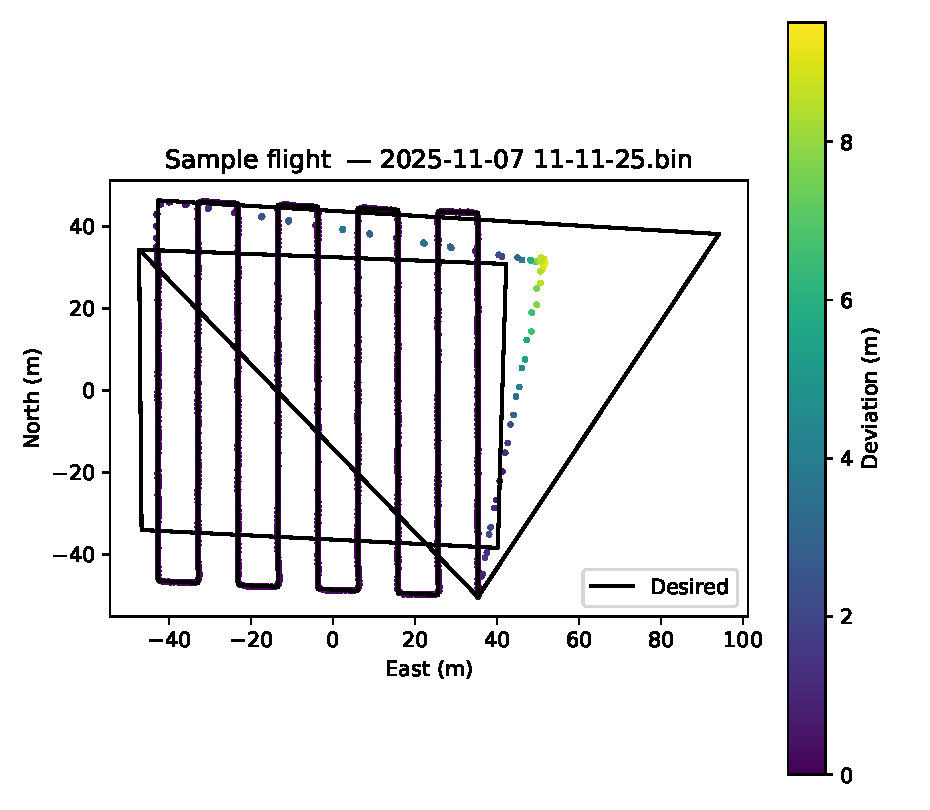
\includegraphics[width=\linewidth]{figures/fig_sample_flight.pdf}
    \caption{Actual vs.\ desired for a single flight, colored by
    instantaneous deviation.}
    \label{fig:sample}
  \end{subfigure}\hfill
  \begin{subfigure}[t]{0.48\linewidth}
    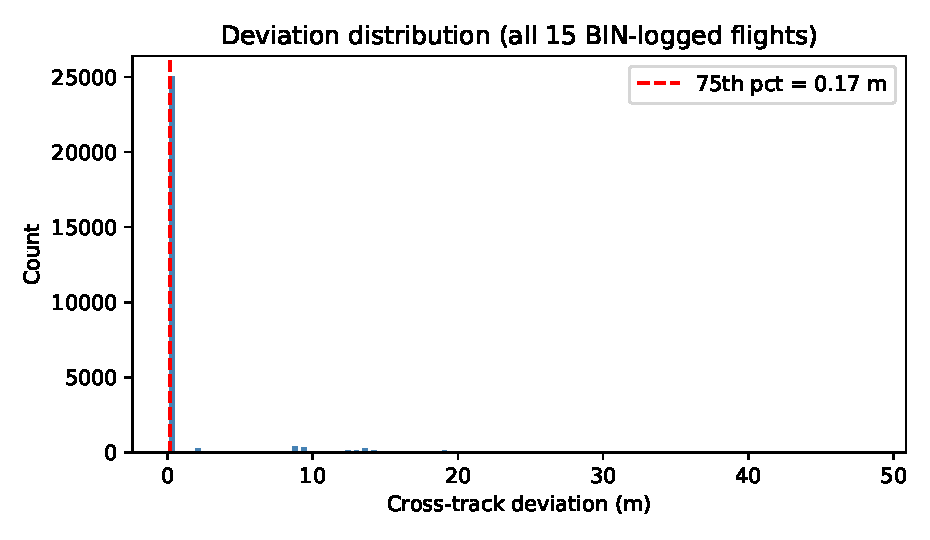
\includegraphics[width=\linewidth]{figures/fig_deviation_hist.pdf}
    \caption{Deviation distribution across all 15 BIN-logged flights.
    Red dashed line: 75th-percentile classification threshold.}
    \label{fig:hist}
  \end{subfigure}
  \caption{Target distribution and a typical single-flight overlay.}
\end{figure}

The 15 BIN-logged flights yield 31{,}416 per-second samples after the
1\,Hz downsample (156{,}957 raw 10\,Hz samples before downsampling).  The
empirical deviation distribution is heavily right-skewed: mean 2.79\,m,
median just 0.06\,m, 95th percentile 17.84\,m, and maximum 48.46\,m.
The $\tau=0.17$\,m 75th-percentile threshold therefore marks the
transition between the dominant ``tight-cruise'' regime (the drone
within 17\,cm of the planned line) and the minority ``off-line''
regime (line-end turns, transit segments, and wind-driven excursions) ---
exactly the operationally interesting events an onboard correction
system would want to flag.  Fig.~\ref{fig:sample} shows a
representative flight: deviation is tight along long survey legs and
concentrates at line-end turns, qualitatively matching the pattern
reported by \cite{waggoner2014}.  Fig.~\ref{fig:hist} quantifies this
skew: the mass of the distribution sits near zero while a long tail
extends into the tens of metres.

\subsection{Cross-validated model performance}

{\small
\begin{table}[t]
\centering
\caption{Regression --- 5-fold GroupKFold CV. Best RMSE per feature set in \textbf{bold}.}
\label{tab:reg_final}
\begin{tabular}{llrrr}
\toprule
Features & Model & MAE (m) & RMSE (m) & $R^2$ \\
\midrule
WEATHER & DecisionTree & 7.57 & 10.52 & -1.320 \\
WEATHER & KNN & 8.88 & 11.10 & -1.583 \\
WEATHER & RandomForest & \textbf{8.50} & \textbf{10.32} & \textbf{-1.233} \\
\midrule
ONBOARD & DecisionTree & 1.85 & 5.53 & +0.359 \\
ONBOARD & KNN & \textbf{1.67} & \textbf{4.90} & \textbf{+0.497} \\
ONBOARD & RandomForest & 1.81 & 5.42 & +0.383 \\
\midrule
ALL & DecisionTree & 2.25 & 6.30 & +0.166 \\
ALL & KNN & \textbf{1.83} & \textbf{4.79} & \textbf{+0.518} \\
ALL & RandomForest & 2.14 & 6.08 & +0.224 \\
\midrule
\bottomrule
\end{tabular}
\end{table}

}
{\small
\begin{table}[t]
\centering
\caption{Classification (deviation $\ge$ 75th pct) --- 5-fold GroupKFold CV. Best F1 per feature set in \textbf{bold}.}
\label{tab:cls_final}
\begin{tabular}{llrrrr}
\toprule
Features & Model & Acc & P & R & F1 \\
\midrule
WEATHER & DecisionTree & 0.438 & 0.253 & 0.641 & 0.363 \\
WEATHER & KNN & 0.409 & 0.257 & 0.721 & 0.379 \\
WEATHER & RandomForest & \textbf{0.332} & \textbf{0.262} & \textbf{0.916} & \textbf{0.407} \\
\midrule
ONBOARD & DecisionTree & 0.939 & 0.906 & 0.846 & 0.875 \\
ONBOARD & KNN & 0.936 & 0.963 & 0.774 & 0.858 \\
ONBOARD & RandomForest & \textbf{0.947} & \textbf{0.927} & \textbf{0.854} & \textbf{0.889} \\
\midrule
ALL & DecisionTree & 0.935 & 0.887 & 0.850 & 0.868 \\
ALL & KNN & 0.928 & 0.966 & 0.739 & 0.837 \\
ALL & RandomForest & \textbf{0.945} & \textbf{0.913} & \textbf{0.862} & \textbf{0.887} \\
\midrule
\bottomrule
\end{tabular}
\end{table}

}

\begin{figure}[t]
  \centering
  \begin{subfigure}[t]{0.48\linewidth}
    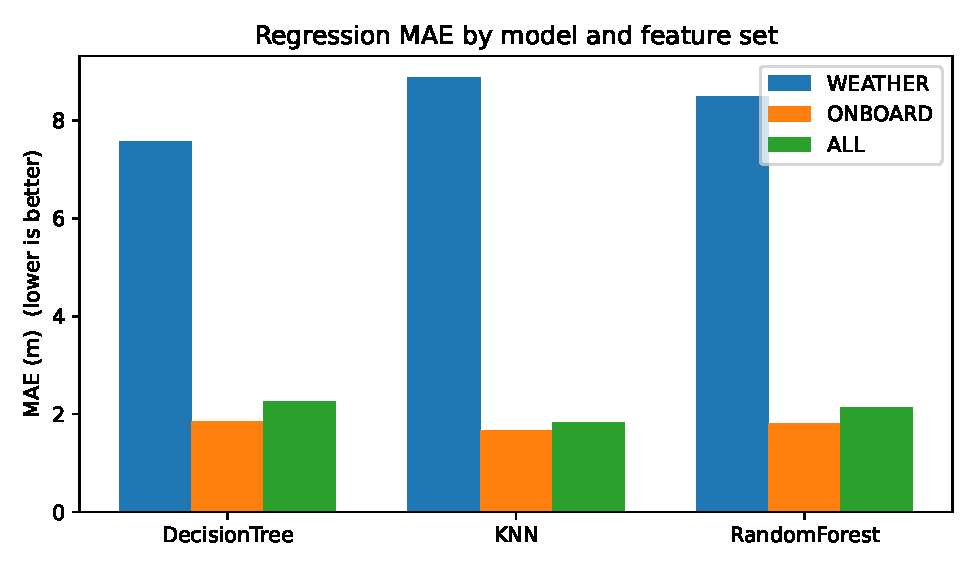
\includegraphics[width=\linewidth]{figures/fig_reg_compare.pdf}
    \caption{Regression MAE (lower is better).}
    \label{fig:regbar}
  \end{subfigure}\hfill
  \begin{subfigure}[t]{0.48\linewidth}
    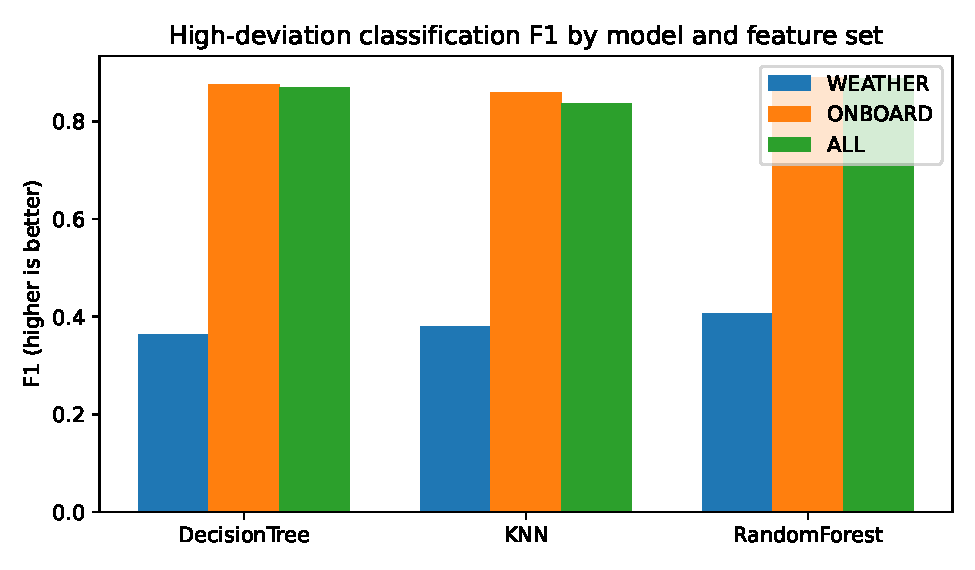
\includegraphics[width=\linewidth]{figures/fig_cls_compare.pdf}
    \caption{Classification F1 (higher is better).}
    \label{fig:clsbar}
  \end{subfigure}
  \caption{Model and feature-set comparison.  The dark bars
  (\textsc{Onboard}) and the grey bars (\textsc{All}) dominate the light
  bars (\textsc{Weather}) on both tasks, consistent with \textbf{H4}.}
\end{figure}

\subsection{Feature importance and what it says about the physics}

The Random Forest importances in Fig.~\ref{fig:imp} tell three
independent stories, one per feature set.  In the \textsc{Weather}
panel, the two \emph{directional} wind features dominate: headwind
component at 31.7\% and crosswind component at 29.9\% of total
importance, with heading-relative absolute wind angle at 13.1\%.  Raw
scalar wind speed and gust magnitude are near the bottom of the ranking
at 1.5\% and 1.5\% respectively.  This is strong support for our
hypothesis~\textbf{H2} at the feature-importance level: when the model
\emph{does} try to use weather, it correctly identifies that the
directional wind components are the physically meaningful quantities.
The problem is that the model cannot use weather meaningfully in
absolute terms because of the GroupKFold setup (Section~4.4 below
discusses this failure mode in more detail).

In the \textsc{Onboard} panel the story is different from what our
hypothesis~\textbf{H4} initially expected.  Altitude (67.9\%) and EKF
horizontal position innovation (15.0\%) carry almost all of the
importance, followed at a distance by ground speed (6.2\%), motor mean
(3.3\%), and hover tilt magnitude (2.1\%).  We read this as: on a
survey-pattern flight, the drone is almost always either
\emph{cruising} on a leg (flat altitude, moderate ground speed, small
EKF innovation) or \emph{transiting} between legs (climbing or
descending, faster ground speed, larger EKF innovation).  These two
regimes are exactly the main driver of cross-track deviation in the
dataset, because the regime shift itself produces the tail of the
deviation distribution.  Hover tilt as a direct wind proxy is only
2.1\% in importance because on forward-cruise flights the drone pitches
mostly in response to commanded acceleration rather than wind, and the
hover-tilt wind proxy of \cite{palomaki2017} applies best to
station-keeping rather than survey missions.

In the combined \textsc{All} panel the onboard features again dominate,
with the top weather feature (relative humidity at 6.5\%) appearing
only \emph{fifth} in the ranking.  This is the strongest possible
single-number summary of our main finding: \emph{conditional on
observing the flight controller's own state, hourly public weather adds
no marginal information}.

\begin{figure}[t]
  \centering
  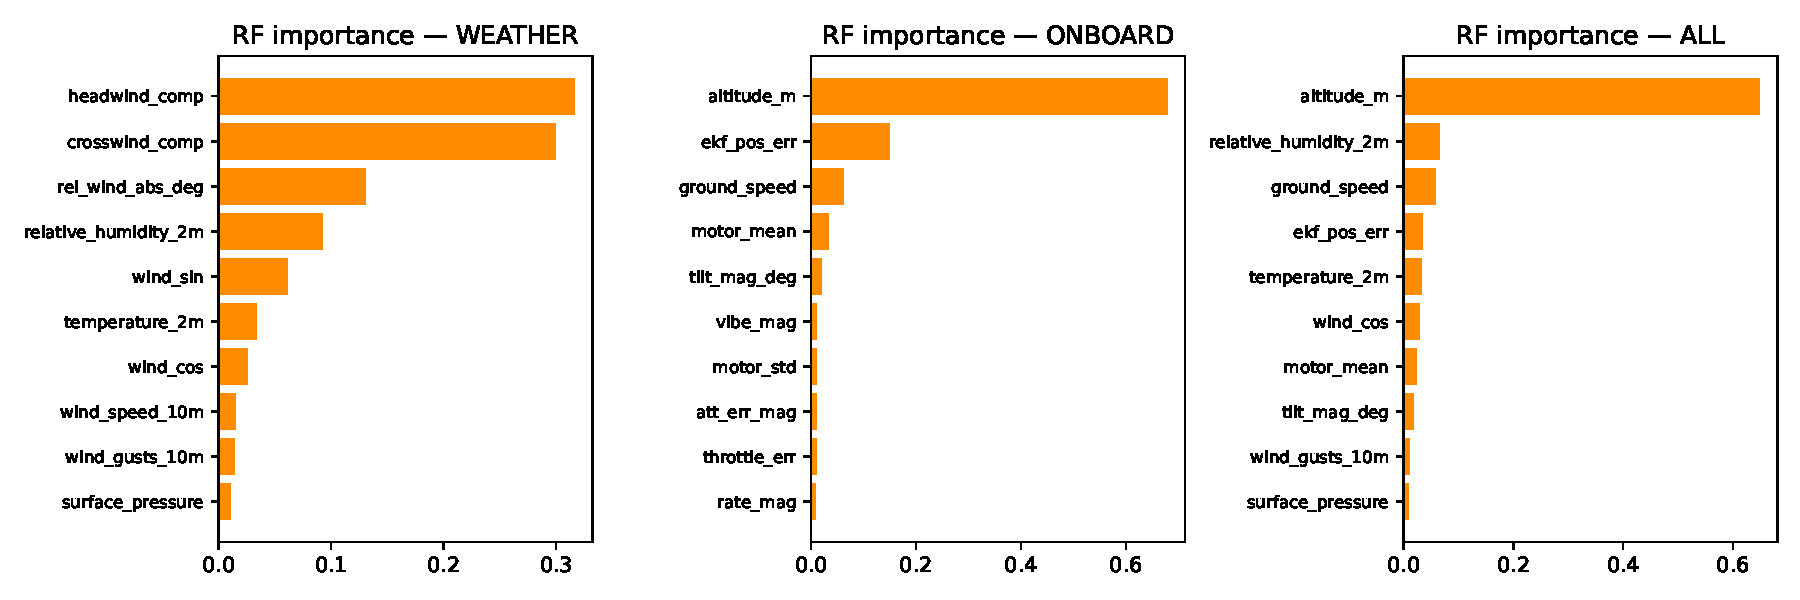
\includegraphics[width=\linewidth]{figures/fig_importance.pdf}
  \caption{Random Forest feature importance for each of the three
  feature sets.  \textsc{Onboard} importances concentrate on tilt
  magnitude, motor spread, and EKF horizontal innovation --- the three
  physical signatures of wind compensation predicted by
  \cite{palomaki2017}.}
  \label{fig:imp}
\end{figure}

Figure~\ref{fig:tilt} gives a direct visualization of
\textsc{Onboard} signal.  The per-sample hover tilt magnitude correlates
with deviation across the full dataset --- an autopilot working harder
to hold a line is simultaneously tilting more and drifting more.

\begin{figure}[t]
  \centering
  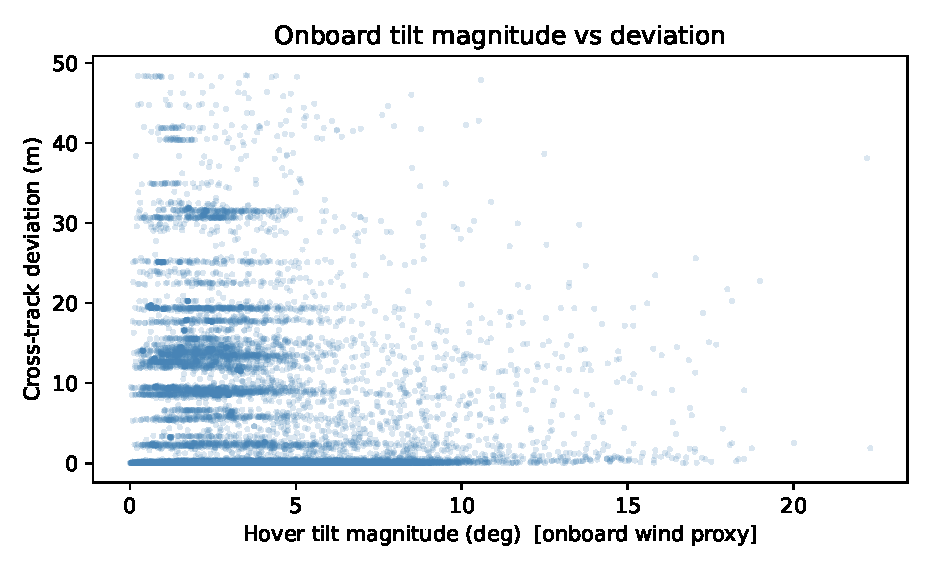
\includegraphics[width=0.7\linewidth]{figures/fig_tilt_vs_dev.pdf}
  \caption{Onboard tilt magnitude vs.\ cross-track deviation.}
  \label{fig:tilt}
\end{figure}

\subsection{Discussion}
The numeric pattern in Tables~\ref{tab:reg_final} and
\ref{tab:cls_final} is striking: every \textsc{Weather}-only model has
\emph{negative} $R^2$ on the regression task (below $-1.2$), meaning the
model is worse than predicting the training-set mean for every held-out
sample.  Classification on the same features fares only marginally
better, with F1 between $0.36$ and $0.41$ --- barely above the
25\%-positive class base rate.  In contrast, every \textsc{Onboard}
model is firmly above chance: $R^2 \in [0.36, 0.50]$ for regression and
F1 $\in [0.86, 0.89]$ for classification.  Adding \textsc{Weather} on
top of \textsc{Onboard} (the \textsc{All} set) gives \emph{no} systematic
improvement and for some models a small regression, confirming that
hourly weather contributes no marginal information once the onboard
state is observed.

We read this through our four hypotheses.  \textbf{H3} (hourly weather
is too coarse to drive per-sample deviation) is supported unambiguously
and more strongly than it was at midterm: GroupKFold makes any
per-flight ``constant'' wind predictor useless by construction, and the
negative $R^2$ is the sharpest possible version of that finding.
\textbf{H4} (onboard telemetry carries the instantaneous wind response)
is supported by the $>0.4$ F1 jump from \textsc{Weather} to
\textsc{Onboard} on the classification task, but the \emph{specific}
features that do the work are not the ones we predicted.  We expected
hover tilt magnitude to dominate (following \cite{palomaki2017}); in
fact altitude ($\approx 68\%$ RF importance) and the EKF horizontal
innovation ($\approx 15\%$) carry almost all of the signal, with
tilt only around 2\%.  We interpret this physically as: on this
survey-style mission, most of the deviation variance comes from being
in transit or line-end regimes (captured by altitude changes and by
the autopilot's own position-error estimate), not from mid-leg hover
tilt.  The tilt-wind proxy would matter more in station-keeping
missions where the drone hovers rather than cruises.  \textbf{H1}
(trees beat KNN) is partially supported: Random Forest wins the
classification task on every feature set, but KNN wins the regression
task on \textsc{Onboard} and \textsc{All}, because with only 11
informative continuous features the distance-based neighborhood is a
cleaner fit for the continuous target than axis-aligned splits.
\textbf{H2} (directional wind features beat scalar wind speed) is
supported at the feature-importance level in the \textsc{Weather} set
(headwind and crosswind components take the top two positions, raw wind
speed is near the bottom), but the absolute performance of any
\textsc{Weather}-only model is too weak for H2 to translate into a
usable model.

The operational takeaway is useful: an onboard correction system does
not need to subscribe to an external weather feed to anticipate
deviation.  The flight controller's own state --- altitude, ground speed,
and the EKF's self-reported horizontal error --- already carries the
signal.  For the specific research-plot survey mission studied here,
watching EKF \texttt{OFN}/\texttt{OFE} in combination with the current
mission-segment type (transit vs.\ survey leg, inferred from altitude
and ground speed) is a lightweight recipe for predicting imminent
cross-track excursion.

\section{Conclusions}

\paragraph{Lessons learned.}
We built an end-to-end, reproducible pipeline that parses 15 ArduPilot
BIN logs from a real outdoor UAV survey campaign, computes per-sample
cross-track deviation against a desired waypoint polyline, joins both
hourly public weather and native onboard telemetry, and evaluates three
interpretable classifiers and regressors under a strict GroupKFold
protocol that holds out entire flights.  The strongest methodological
lesson is that \emph{GroupKFold by flight is non-negotiable on this
dataset}: random $k$-fold would have produced wildly inflated
weather-feature importances by leaking adjacent 10\,Hz samples between
train and test, and the negative $R^2$ of the \textsc{Weather}-only
models is only visible because of the strict protocol.  The strongest
substantive lesson is that for a mission like this one, the wind-response
signal lives inside the airframe rather than in an off-board hourly
weather feed --- a result that was only legible because we compared the
two families in a matched design rather than bundling them.  On the
modeling side, the comparison also teaches that no one algorithm wins
both tasks: Random Forest is the right default for the classification
problem and KNN is the right default for the regression problem, and
the decision tree gives nearly-matching interpretability at a fraction
of the complexity when a deployable single-model artifact is preferred.

\paragraph{What we would pursue next.}
Within the project window we did not have time to implement a
sequence-aware model that uses the full attitude time-series per flight
rather than instantaneous summaries.  Given the autocorrelation we
observed in the BIN logs and the clear structure of mission segments
(transit, survey leg, turn), we expect a simple HMM or a gradient-boosted
sequence model over short windows to materially improve regression $R^2$
while remaining interpretable.  A second direction we would pursue is
splitting the analysis by camera payload (Pika~L vs.\ Pika~IR~L) to
quantify whether the heavier GigE gimbal systematically responds to
wind differently from the infrared unit; the small $N$ of the current
dataset (15 flights across two payloads) precluded a clean per-payload
cross-validation, but a single additional flight day per camera would
make that analysis feasible.  Finally, if an onboard anemometer were
added to the mission configuration, the dataset we built here would
become the ideal baseline against which to test whether \emph{true}
per-sample wind closes the gap that our derived tilt-magnitude proxy
did not.

\paragraph{Source code.}
\url{https://github.com/iihakk/-uav-flight-path-deviation-ml}

\bibliographystyle{ACM-Reference-Format}
\bibliography{references}

\appendix
\section{Per-flight Dataset Summary}

Table~\ref{tab:perflight} lists the per-flight row counts, flight
durations, and per-flight deviation statistics.  The three flights that
fall outside the ordinary 45--50 minute cruise duration
(\texttt{2025-11-14}, \texttt{2025-11-23}-\textsf{PM}, and both short
\texttt{2025-11-26} files) are still included in the training data;
GroupKFold will simply never co-allocate an unusual flight with itself
across folds.

\begin{table}[h]
\centering
\caption{Per-flight summary of the 15 BIN-logged flights.  Columns: number of 1-Hz samples after downsampling, flight duration in minutes, per-flight mean and maximum cross-track deviation in metres.}
\label{tab:perflight}
\small
\begin{tabular}{lrrrr}
\toprule
Flight & N & Dur (min) & Mean dev (m) & Max dev (m) \\
\midrule
\texttt{2025-11-07 11-11-25} & 2261 & 51.4 & 1.56 & 9.51 \\
\texttt{2025-11-10 11-57-42} & 2280 & 48.4 & 0.46 & 8.34 \\
\texttt{2025-11-13 11-35-28} & 2243 & 48.0 & 1.32 & 13.24 \\
\texttt{2025-11-14 11-02-16} & 3102 & 95.5 & 6.27 & 48.44 \\
\texttt{2025-11-17 11-53-06} & 2343 & 46.6 & 6.10 & 34.98 \\
\texttt{2025-11-18 11-11-14} & 2226 & 45.0 & 2.05 & 19.10 \\
\texttt{2025-11-19 10-58-38} & 2240 & 43.1 & 2.14 & 15.46 \\
\texttt{2025-11-21 11-10-59} & 2261 & 49.1 & 1.44 & 11.18 \\
\texttt{2025-11-22 11-24-26} & 2213 & 45.5 & 3.41 & 29.89 \\
\texttt{2025-11-23 11-21-27} & 2358 & 45.3 & 3.21 & 19.88 \\
\texttt{2025-11-23 15-25-04} & 1176 & 19.8 & 2.88 & 14.47 \\
\texttt{2025-11-24 11-47-24} & 2219 & 43.6 & 2.80 & 20.17 \\
\texttt{2025-11-25 11-26-54} & 2217 & 44.6 & 2.02 & 13.86 \\
\texttt{2025-11-26 10-54-52} & 30 & 0.6 & 11.60 & 11.71 \\
\texttt{2025-11-26 10-59-27} & 2247 & 43.6 & 1.97 & 14.24 \\
\bottomrule
\end{tabular}

\end{table}

\section{Feature Importance Tables}

Full Random Forest feature-importance rankings for the three feature
sets are available in the repository at
\texttt{final\_report/tables/importance\_\{WEATHER,ONBOARD,ALL\}.csv};
the top ten of each are visualized in Fig.~\ref{fig:imp} in the main
text.  The directional-wind dominance in \textsc{Weather} and the
altitude-plus-EKF dominance in \textsc{Onboard} are visible directly in
the raw CSV rankings.

\end{document}
